\documentclass{article}
\usepackage[utf8]{inputenc}

\title{Distilling the knowledge in a neural network}
\author{}
\date{}

\usepackage{natbib}
\usepackage{graphicx}
\usepackage{amsmath}
\usepackage[left=2.5cm,right=2.5cm,top=1cm,bottom=1.25cm]{geometry}
\usepackage{hyperref}
\hypersetup{colorlinks=true,urlcolor=blue}
\pagenumbering{gobble}

\begin{document}

\maketitle

\section*{Link}
\href{https://arxiv.org/abs/1503.02531}{arxiv} 

\section*{Summary}
\begin{itemize}
    \item We can train very cumbersome models(ensemble of separately trained models or a single very large model with strong regularizer) to extract structure from very large, highly redundant datasets. But during deployment we have more stringent requirements on latency and computational resources. To address this we will use a different kind of training(distillation) to transfer knowledge from the cumbersome model to to a small model that is more suitable for deployment. 
    \item When we use maximum log likelihood criterion as training objective, the trained model assigns probabilities to all the classes. Even when the probabilities for wrong classes are very small their relative probability tend to be significant. For example a model may assign a very small probability to an image of BMW being garbage truck but it will still usually be much higher than the probability of being a carrot. This tells us a garbage truck is more similar to a BMW than a carrot is to a BMW. This kind of information shows how a cumbersome model tend to generalize which is missing when we use hard target(like one hot encoding) for training.
    \item One way to transfer the generalization ability of the cumbersome model to a small model is to use the class probabilities produced by the cumbersome model as soft targets for training the small model. When these soft targets have higher entropy they provide more information per training case than hard targets and much less variance in the gradient between training cases, so the small model can often be trained on much less data than the original cumbersome model and using a much higher learning rate. The problem with this approach is that the assigns probabilities are usually too low (specially for task like MNIST) for the wrong classes to have significant effect on cross entropy error(remember cross entropy loss is $\sum_{y} y_{true} \log y_{pred}$, here $y_{true}$ will be the soft target from cumbersome model and $y_{pred}$ the probability obtained from simpler model). One way to circumvent this is to use the logits(input to final softmax) as the target for simple model (which will have larger contribution for small values compared to their softmax output).  
    \item In this paper they propose a solution that raise the temperature term $T$ in general softmax equation
    \begin{equation*}
        q_i = \dfrac{exp(z_i/T)}{\sum_{j}exp(z_j/T)}
    \end{equation*}
    Raising the temperature produces a softer output as can be seen in \autoref{fig:Figure 1}. This means smaller logits will have relatively more contribution to the cross entropy error.
    \begin{figure}
        \centering
        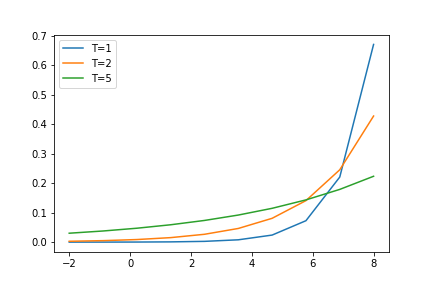
\includegraphics{softmax_temperature.png}
        \caption{Effect of temperature on softmax output}
        \label{fig:Figure 1}
    \end{figure}
    \item For training they use two objective functions:
    \begin{enumerate}
        \item Cross entropy with the soft target from cumbersome model, using the same high temperature as the complex model.
        \item Cross entropy with correct labels(one hot encoding) but with temperature 1. 
    \end{enumerate}
    The total loss is then a weighted average of those two losses. The second loss is given considerably lower weight than the first one. Magnitude of gradient produced by first objective function scales as $1/T^2$. So we multiply them by $T^2$ so that relative contributions of the soft and hard target remain roughly unchanged if $T$ is changed.
    \item Experiment is done on MNIST using a neural net with two hidden layers of 1200 rectified linear units with dropout regularizer as the cumbersome model and a neural net with two hidden layers of 800 rectified linear units and no regularization as smaller model. The larger model achieved 67 test errors. The smaller model achieved 146 test errors when trained using hard targets. But then the objective function include soft target as well the smaller model achieved 74 test errors. Thus showed that the soft targets can transfer a great deal of generalization knowledge to the distilled model.  
    \item Experiment on Automatic Speech Recognition(ASR) system shows that the distilled model is able to achieve much better performance than a model trained on hard labels and can approximate performance gained by using a ensemble of 10 models.
    \item When the dataset is very large or the individual models are large we can train several specialist models that that each focus on a different confusable subset of the classes. Using soft targets for the specialists can reduce the overfitting. Specialist models are much faster to train than large ensembles and improves performance.
    \item Soft targets can act as a regularizer and is a very effective way of communicating the regularities discovered by a model trained on all of the data to another model(possibly trained on fewer data).
\end{itemize}

\end{document}
